\setchapterimage[8cm]{Paul Pastourmatzis Unsplash}
\setchapterpreamble[u]{\margintoc}
\chapter{commutative alegbra}
\labch{commutative_algebra}
% in English

The reference book is \cite{Atiyah}.

The following "ring" means a commutative ring with unity.

\section{Basic concepts}

% Inclusion of sets is denoted by $\subseteq$. We reserve the sign $\subset$ for strict inclusion.

% A zero-divisor in a ring $A$ is an element $x$ which "divides 0", i.e., for which there exists $y\ne 0$ in $A$ such that $xy=0$. A ring without non-zero zero-divisors is called an integral domain.\sidenote{For exmaple, $\mathbb{Z}$ and $\mathbb{k}[x_1,...,x_n]$ are integral domains.}

% An element $x$ of a ring $A$ is called nilpotent if there exists $n\in \mathbb{N}$ such that $x^n=0$. A nilpotent element is a fortiori\sidenote{a fortiori: 显然地(拉丁语)} a zero-divisor, but not conversely in general.

% A unit in $A$ is an element $x$ which "divides 1", i.e., for which there exists $y\in A$ such that $xy=1$. The set of units in $A$ is denoted by $A^\times$.\sidenote{The units form an abelian group under multiplication.}

% The multiples $ax$ of an element $x\in A$ form a principal ideal, denoted by $(x)$ or $Ax$. $x$ is a unit if and only if $(x)=A=(1)$. 

% The zero ideal $(0)$ is usually denoted by $0$.

% \begin{proposition}
%     Let $A$ be a non-zero ring. TFAE:
%     \begin{enumerate}
%         \item $A$ is a field.
%         \item the only ideals in $A$ are $(0)$ and $(1)$.
%         \item every homomorphism $A\to B$ of rings with unity is injective.
%     \end{enumerate}
% \end{proposition}

\begin{align*}
    \mathfrak{p} \text{ is prime} & \iff A/\mathfrak{p} \text{ is an integral domain}\\
    \mathfrak{m} \text{ is maximal} & \iff A/\mathfrak{m} \text{ is a field}
\end{align*}
The zero ideal is prime if and only if $A$ is an integral domain.
\begin{note}
    Prime ideals are fundamental in the study of commutative algebra.
\end{note}
\begin{theorem}
    Every ring $A\ne 0$ has at least one maximal ideal.
\end{theorem}
\begin{proof}
    This is a consequence of Zorn's lemma. See \cite{Atiyah} p.4.
\end{proof}
\begin{proposition}
    The set $\mathfrak{R}$\footnote{The ideal $\mathfrak{R}$ is called the \textit{nilradical} of $A$.} of all nilpotent elements of $A$ is an ideal, and $A/\mathfrak{R}$ is reduced, i.e., has no non-zero nilpotent elements.
\end{proposition}
\begin{proof}
    照章办事. See \cite{Atiyah} p.5.
\end{proof}
\begin{proposition}
    The nilradical of $A$ is the intersection of all prime ideals of $A$.
\end{proposition}
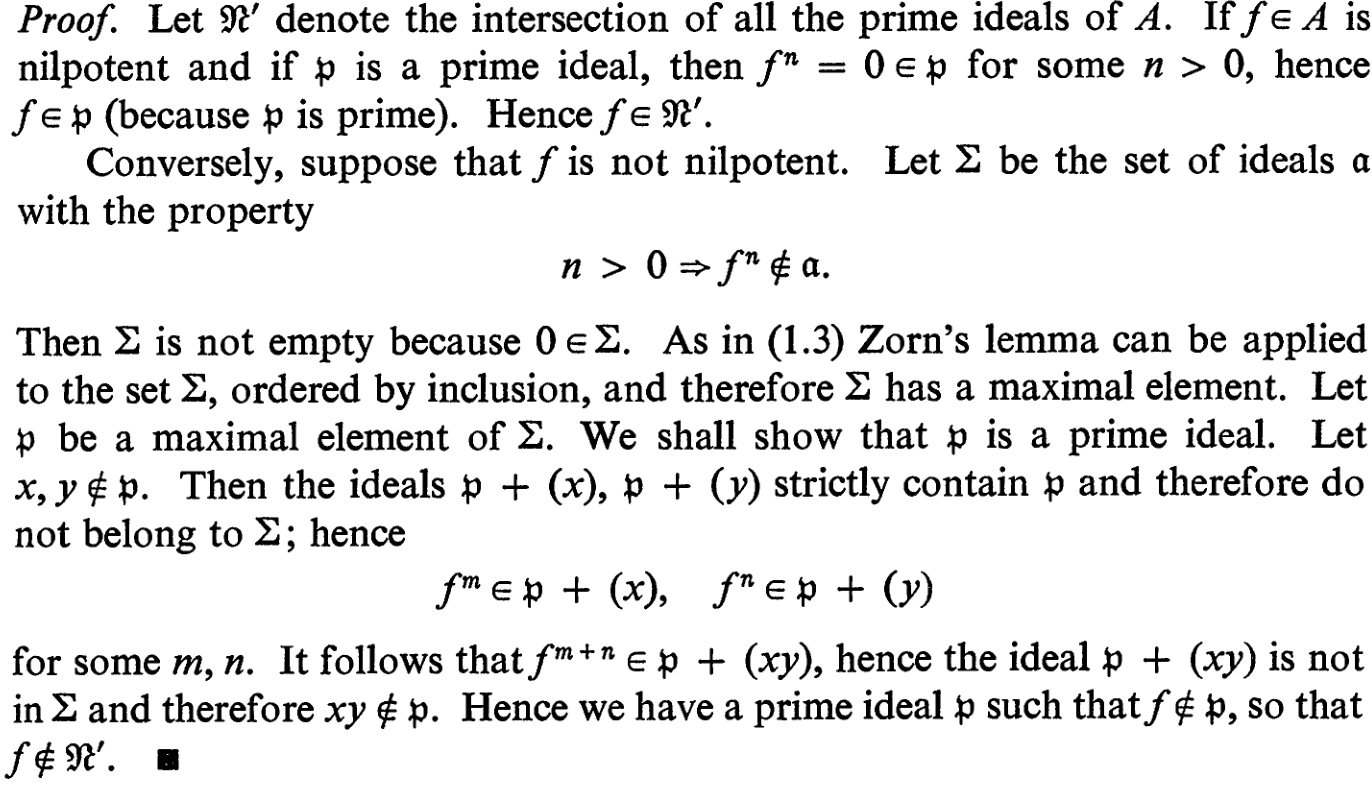
\includegraphics[width=\textwidth]{figures/image.png}

The Jacobson radical $\mathfrak{R}$ of $A$ is the intersection of all maximal ideals of $A$.

\begin{proposition}
    $x\in \mathfrak{R}$ if and only if $1-xy$ is a unit for all $y\in A$.
\end{proposition}
\includegraphics[width=\textwidth]{figures/image copy.png}









\begin{thebibliography}{99}
    \bibitem{Atiyah}
    Atiyah, M. F. (1969). \textit{Introduction to Commutative Algebra}. Addison-Wesley.
\end{thebibliography}
